\begin{frame}
    \frametitle{Experiments}
    \framesubtitle{Integrator scaling}

\begin{figure}[H]
    \centering
    \label{fig:time}
    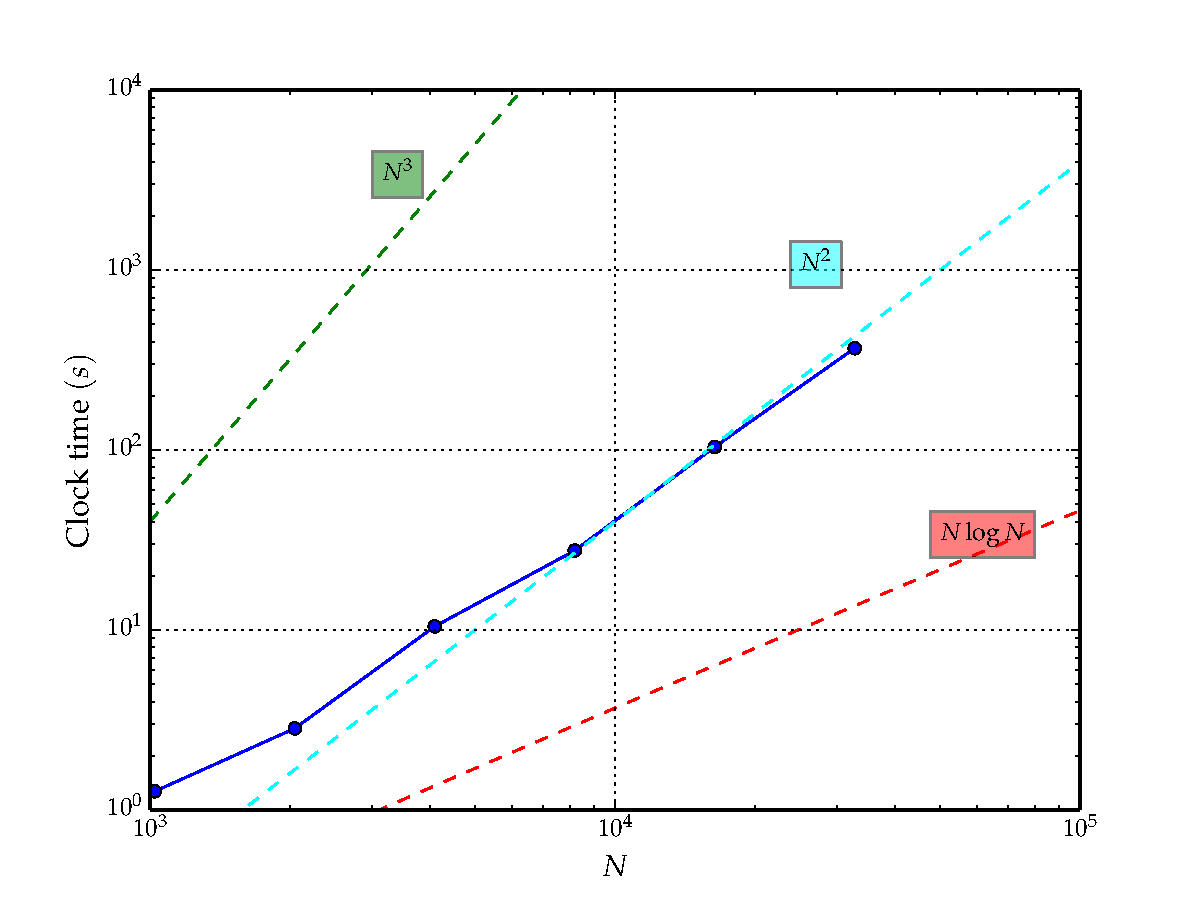
\includegraphics[width=0.65\textwidth]{img/test_time-1t-N.pdf}
    \caption{Clock time of integration up to $t=1$ NBU using $\eta = 0.01$ and
             $\epsilon = 10^{-4}$ using different amount of particles.}
\end{figure}

\end{frame}
\begin{frame}
    \frametitle{Experiments}
    \framesubtitle{Clock time comparison}

\begin{table}[H]
    \centering
    \footnotesize
    \begin{tabular}{rrrrr}
        \hline
        {\bf N} & \multicolumn{1}{c}{\bf CPU}
                & \multicolumn{1}{c}{\bf CPU + OpenMP}
                & \multicolumn{1}{c}{\bf CPU + GPU}
                & \multicolumn{1}{c}{\bf GPU}   \\
                & (single thread) & (many threads)     & (mixed approach) &  (multi threads) \\ \hline
         {\bf  1k} &    12.98 [s] &   8.19 [s] &    3.57 [s]           &    1.21 [s]          \\
         {\bf  2k} &    61.32 [s] &  34.94 [s] &   13.42 [s]           &    3.22 [s]          \\
         {\bf  4k} &   282.98 [s] & 162.64 [s] &   54.28 [s]           &    9.45 [s]          \\
         {\bf  8k} &  1227.40 [s] & 682.56 [s] &  208.91 [s]           &   23.31 [s]          \\
         {\bf 16k} &  5542.35 [s] & 3227.91 [s] &  904.82 [s]           &   82.63 [s]          \\
         {\bf 32k} & 26383.71 [s] & 15076.40 [s] & 3722.92 [s]           &  275.53 [s]          \\ \hline
    \end{tabular}
    \caption{Clock time foreach integrator version.}
    \label{tab:acc}
\end{table}

\end{frame}

\begin{frame}
    \frametitle{Experiments}
    \framesubtitle{Clock time comparison}

\begin{figure}[H]
    \centering
    \label{fig:acc}
    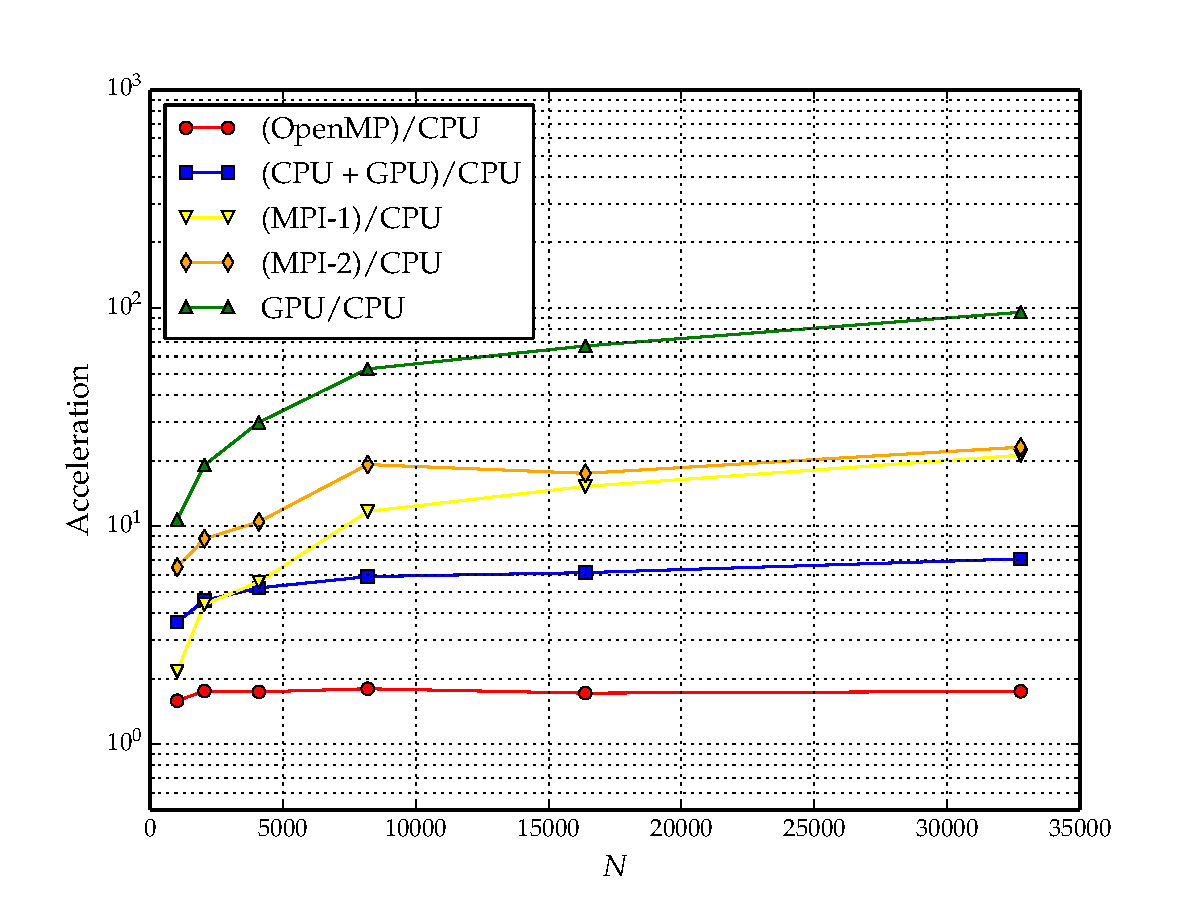
\includegraphics[width=0.7\textwidth]{img/test_gpu-acceleration.pdf}
    \caption{Acceleration between the implementations described in Table~\ref{tab:acc}}
\end{figure}

\end{frame}
\begin{frame}
    \frametitle{Experiments}
    \framesubtitle{Integrator Performance}
\begin{figure}[H]
    \centering
    \label{fig:gflops}
    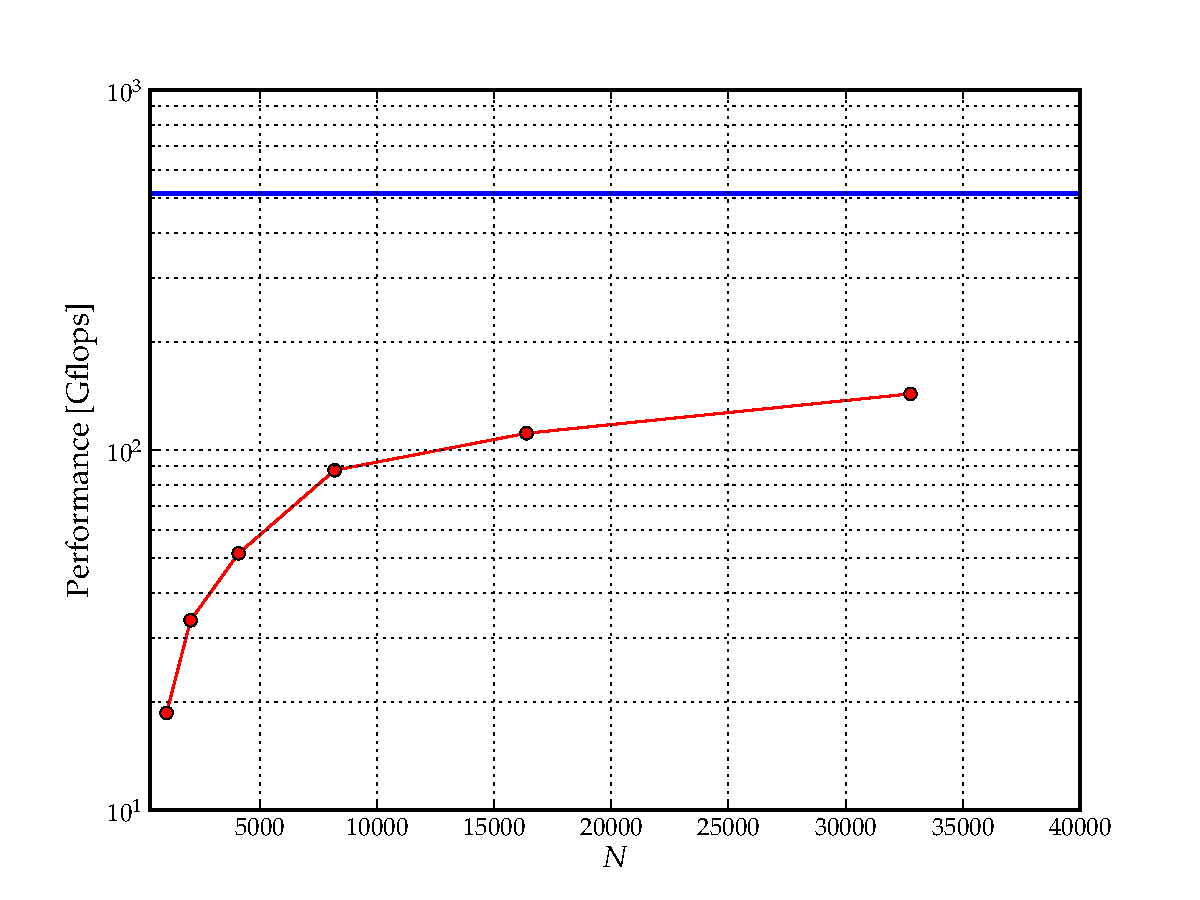
\includegraphics[width=0.65\textwidth]{img/test_gflops.pdf}
    \caption{GPU gravitational interactions performance in GFLOPS for different amount of particles.}
\end{figure}

\end{frame}
